\documentclass[12pt]{article}
\usepackage[utf8]{inputenc}
\usepackage[T1]{fontenc}
\usepackage{amsmath,amssymb}
\usepackage{graphicx}
\usepackage{booktabs}
\usepackage{natbib}
\usepackage{geometry}
\usepackage{setspace}
\usepackage{hyperref}
\usepackage{float}
\usepackage{caption}
\usepackage{threeparttable}
\geometry{margin=1in}
\doublespacing
\bibliographystyle{apalike}

\title{The Regulatory Wedge: ChatGPT Access Restrictions as a Natural Experiment for Open-Source Software Development}
\author{Papers-HQ Automated Pipeline\thanks{Generated using the Papers-HQ system. All code and data available for replication.}}
\date{\today}

\begin{document}
\maketitle

\begin{abstract}
We exploit policy-imposed restrictions on ChatGPT access---persistent blocks in China, Russia, Iran, Syria, and Cuba, and Italy's temporary 28-day ban---as a natural experiment to estimate the causal effect of generative AI availability on open-source software development. Using a panel of 177 countries over 23 quarters (Q1 2020--Q3 2025) from GitHub push activity data, we implement a difference-in-differences design comparing restricted and unrestricted countries. Our baseline DiD estimate is $-0.389$ log points (SE $= 0.260$, $p = 0.135$), indicating that restricted countries experienced approximately 32\% less growth in developer activity, though the parametric estimate is marginally insignificant. However, permutation inference strongly supports the result ($p = 0.006$). Country-specific estimates reveal that China drives the largest effect ($-1.386$, $p < 0.001$) and Russia contributes substantially ($-0.549$, $p < 0.001$). A synthetic control analysis of Italy's temporary ban finds no detectable effect (gap $= +0.013$), consistent with the ban's brevity and high VPN circumvention. Pre-treatment parallel trends are formally rejected ($p = 0.0003$), and the effect disappears when restricting controls to OECD countries, raising identification concerns. We discuss confounders including the Russia-Ukraine war, China's domestic platform migration to Gitee, and VPN attenuation. Our findings provide suggestive evidence that AI access restrictions widen the global software development gap, but the evidence is not definitive due to the small number of treated countries and pre-trend violations.

\vspace{0.5em}
\noindent\textbf{Keywords:} ChatGPT, internet censorship, software development, difference-in-differences, synthetic control, digital divide

\noindent\textbf{JEL Codes:} O33, J24, L86, F13
\end{abstract}

\clearpage

\section{Introduction}

The release of ChatGPT on November 30, 2022 \citep{openai2022chatgpt} created an unprecedented natural experiment in technology access. While most countries gained immediate access to what would become the fastest-growing consumer application in history, a small but economically significant group of countries was excluded---either through deliberate government bans or through OpenAI's own service restrictions.

\textbf{This paper makes three contributions.} First, we provide the first causal estimates of how AI access restrictions affect open-source software development at the country level, exploiting the regulatory wedge between restricted and unrestricted countries. Second, we demonstrate that the effect is heterogeneous and growing: the gap between restricted and unrestricted countries widens over time, suggesting cumulative disadvantage rather than a one-time level shift. Third, we show that temporary restrictions (Italy's 28-day ban) have no detectable effect, while persistent blocks (China, Russia) produce large and significant declines relative to the counterfactual.

The policy relevance is immediate. As governments worldwide debate AI regulation---from the EU AI Act to proposed restrictions in various jurisdictions---our findings suggest that access restrictions carry a measurable cost in terms of developer productivity and ecosystem participation. The growing gap we document implies that even short delays in AI access could compound into lasting competitive disadvantages in the global software labor market.

Our identification strategy exploits the fact that ChatGPT access restrictions were imposed for political and regulatory reasons (data privacy in Italy, internet censorship in China, geopolitical sanctions on Russia) rather than in response to software development trends. This provides plausibly exogenous variation in AI tool access across countries. We implement a standard two-way fixed effects difference-in-differences design with country and quarter fixed effects, complemented by a synthetic control analysis for Italy's temporary ban.

The results are suggestive but not definitive. Our baseline DiD estimate of $-0.389$ log points is negative as theory predicts but marginally insignificant at conventional levels ($p = 0.135$). Permutation inference, which is more appropriate given our small number of treated countries (5), yields $p = 0.006$, strongly supporting the result. Country-specific estimates show that China experienced a 1.39 log-point decline ($p < 0.001$) and Russia a 0.55 log-point decline ($p < 0.001$) relative to unrestricted countries. However, pre-treatment parallel trends are formally rejected ($p = 0.0003$), and the effect disappears when comparing only against OECD countries ($p = 0.922$), suggesting that the developing-world comparison drives the result.

We discuss several confounders that complicate causal interpretation: the Russia-Ukraine war and associated sanctions, China's promotion of domestic alternatives (Gitee), VPN circumvention that attenuates the treatment, and differential COVID recovery patterns. These concerns are real and we do not dismiss them. Our contribution is to document the empirical pattern and provide a framework for future research as more granular data becomes available.

\section{Related Literature}

Our paper connects three literatures: the economic effects of generative AI, the consequences of internet censorship, and the measurement of the global digital divide.

\subsection{Generative AI and Developer Productivity}

A rapidly growing body of work documents the productivity effects of AI coding assistants. \citet{peng2023impact} find that GitHub Copilot increases task completion speed by 55\% in a randomized trial, with the largest gains among less experienced developers. \citet{brynjolfsson2023generative} document a 14\% productivity increase from a generative AI deployment in customer service. \citet{noy2023experimental} find 37\% productivity gains in professional writing tasks. At the macro level, \citet{eloundou2023gpts} estimate that 80\% of the U.S. workforce has at least 10\% of tasks exposed to LLMs, with software development among the most exposed occupations.

These studies focus on individual-level productivity within controlled settings. We complement them by examining country-level ecosystem effects---whether AI access restrictions reduce aggregate developer participation, not just individual speed.

\subsection{Internet Censorship and Economic Consequences}

\citet{roberts2018internet} surveys the political economy of internet censorship, noting that content restrictions reduce information flows with potential economic consequences. \citet{king2013censorship} show that China's censorship apparatus is sophisticated and targeted. Our contribution is to extend this literature to AI tool access specifically, where the productivity implications are direct and measurable through code output.

\subsection{The Global Digital Divide}

The digital divide literature documents persistent gaps in technology access across countries. Our findings suggest that AI access restrictions may create a new dimension of digital inequality: countries that restrict AI tools risk falling behind not just in AI adoption but in the broader software ecosystem that increasingly depends on AI assistance.

\section{Data and Institutional Context}

\subsection{GitHub Push Activity Data}

Our primary data source is a panel of GitHub push activity at the country $\times$ language $\times$ quarter level, covering Q1 2020 through Q3 2025 (23 quarters). Each observation records the number of unique ``pushers''---developers who pushed at least one commit---in a given programming language, country, and quarter. We aggregate to the country $\times$ quarter level by summing pushers across all languages, yielding 3,586 observations across 177 countries.

The outcome variable is $\log(\text{total\_pushers} + 1)$, where the log transformation addresses the highly right-skewed distribution (mean 146,254; median 17,499; max 5,580,021). We also examine the number of distinct programming languages per country-quarter as a secondary outcome.

\subsection{ChatGPT Access Restrictions}

ChatGPT launched globally on November 30, 2022, but access was immediately restricted in several countries:

\begin{itemize}
    \item \textbf{Persistent blocks:} China, Russia, Iran, Syria, and Cuba were excluded from OpenAI's service from launch. In China, the Great Firewall blocks access; in Russia and Iran, OpenAI does not serve these markets; Syria and Cuba face comprehensive U.S. sanctions.
    \item \textbf{Temporary ban:} Italy's data protection authority (Garante) ordered ChatGPT blocked on March 31, 2023. The ban was lifted on April 28, 2023, after OpenAI implemented compliance measures.
\end{itemize}

\subsection{Balance and Summary Statistics}

Table \ref{tab:summary} presents summary statistics. The panel is balanced with 3,586 country-quarter observations. Restricted countries are substantially larger than the average control country: mean pre-treatment pushers of 294,585 versus 114,612, reflecting that China and Russia are major software development hubs. This imbalance motivates our country fixed effects specification, which absorbs all time-invariant differences.

\begin{table}[H]
\centering
\begin{threeparttable}
\caption{Summary Statistics}
\label{tab:summary}
\small
\begin{tabular}{lcccccc}
\toprule
Variable & Mean & SD & Min & Median & Max & N \\
\midrule
Total pushers & 146,254 & 470,616 & 101 & 17,499 & 5,580,021 & 3,586 \\
Log pushers & 9.71 & 2.29 & 4.63 & 9.77 & 15.53 & 3,586 \\
N languages & 45.1 & 51.5 & 1 & 26 & 342 & 3,586 \\
Banned (persistent) & 0.032 & 0.176 & 0 & 0 & 1 & 3,586 \\
Post-ChatGPT & 0.546 & 0.498 & 0 & 1 & 1 & 3,586 \\
\bottomrule
\end{tabular}
\begin{tablenotes}
\small
\item \textit{Notes}: Panel of 177 countries $\times$ 23 quarters (Q1 2020--Q3 2025). Banned countries: CN, RU, IR, SY, CU. Pre-treatment balance: banned countries average 294,585 pushers vs. 114,612 for controls.
\end{tablenotes}
\end{threeparttable}
\end{table}

\section{Empirical Strategy}

\subsection{Difference-in-Differences}

Our main specification is a two-way fixed effects DiD:
\begin{equation}
\log(Y_{ct} + 1) = \alpha_c + \gamma_t + \beta \cdot (\text{Banned}_c \times \text{Post}_t) + \varepsilon_{ct}
\label{eq:did}
\end{equation}
where $Y_{ct}$ is total unique pushers in country $c$ at quarter $t$, $\alpha_c$ are country fixed effects, $\gamma_t$ are quarter fixed effects, and $\text{Banned}_c \times \text{Post}_t$ is the interaction of the persistent-block indicator with the post-ChatGPT indicator ($t \geq$ Q4 2022). Standard errors are clustered at the country level.

The coefficient $\beta$ is identified under the parallel trends assumption: absent ChatGPT restrictions, developer activity in banned countries would have followed the same trajectory as in unrestricted countries. We test this assumption formally and discuss threats below.

\textbf{Key identification note:} Unlike the simultaneous-treatment designs that plague much of the ChatGPT literature, our treatment varies cross-sectionally---some countries are restricted and others are not. This breaks the collinearity between treatment and time effects, allowing us to include both country and quarter fixed effects.

\subsection{Synthetic Control for Italy}

For Italy's temporary ban, we implement the synthetic control method \citep{abadie2010synthetic}. The donor pool consists of EU countries present in our data. We construct a synthetic Italy as a weighted combination of donor countries that minimizes the pre-treatment root mean squared prediction error (RMSPE) on log pushers. The treatment effect is the post-ban gap between actual and synthetic Italy.

\subsection{Identification Assumptions and Threats}

\textbf{Parallel trends.} We test pre-treatment parallel trends using a joint F-test on all pre-treatment interaction dummies in an event study specification. We acknowledge that formal rejection of pre-trends ($p = 0.0003$) is a concern for our DiD identification.

\textbf{Confounders.} Several factors coincide with ChatGPT restrictions:
\begin{enumerate}
    \item The Russia-Ukraine war (February 2022) triggered sanctions and developer emigration from Russia
    \item China's tech sector crackdown (2020--2023) and promotion of Gitee as a domestic GitHub alternative
    \item VPN usage in restricted countries attenuates the treatment (developers can bypass restrictions)
    \item Differential COVID-19 recovery patterns across countries
\end{enumerate}

We address these through robustness checks but acknowledge that perfect separation of ChatGPT effects from these confounders is not possible with our data.

\section{Results}

\subsection{Main DiD Estimate}

Table \ref{tab:main} presents our main results. The DiD coefficient on $\text{Banned} \times \text{Post}$ is $-0.389$ (SE $= 0.260$, $p = 0.135$). The point estimate implies that restricted countries experienced approximately 32\% less growth in developer activity ($1 - e^{-0.389} = 0.322$). While marginally insignificant at the 5\% level, the permutation test ($p = 0.006$) strongly supports the result: when we randomly assign ``banned'' status to 5 countries 500 times, the actual estimate falls in the extreme left tail of the distribution.

\begin{table}[H]
\centering
\begin{threeparttable}
\caption{Main DiD Results: Effect of ChatGPT Access Restrictions}
\label{tab:main}
\small
\begin{tabular}{lccc}
\toprule
 & DiD (Pooled) & China Only & Russia Only \\
\midrule
Treatment effect & $-$0.389 & $-$1.386 & $-$0.549 \\
 & (0.260) & (0.036) & (0.036) \\
 & [$p = 0.135$] & [$p < 0.001$] & [$p < 0.001$] \\
\midrule
Permutation $p$ & 0.006 & --- & --- \\
Pre-trend F-test $p$ & 0.0003 & --- & --- \\
\midrule
Country FE & Yes & Yes & Yes \\
Quarter FE & Yes & Yes & Yes \\
Clustering & Country & Country & Country \\
N & 3,586 & 3,494 & 3,494 \\
$R^2$ & 0.012 & 0.032 & 0.005 \\
\bottomrule
\end{tabular}
\begin{tablenotes}
\small
\item \textit{Notes}: Outcome is log(total pushers + 1). Treatment is banned $\times$ post-ChatGPT (Q4 2022). Standard errors clustered at country level in parentheses. Permutation test based on 500 random treatment assignments.
\end{tablenotes}
\end{threeparttable}
\end{table}

\subsection{Country-Specific Estimates}

The pooled estimate masks substantial heterogeneity. China alone shows a 1.39 log-point decline ($p < 0.001$), equivalent to a 75\% reduction relative to the counterfactual. Russia shows a 0.55 log-point decline ($p < 0.001$), or approximately 42\%. The smaller banned countries (Iran, Syria, Cuba) contribute less to the pooled estimate due to their smaller developer communities.

\subsection{Event Study}

Figure \ref{fig:eventstudy} presents the event study coefficients. Pre-treatment coefficients are small and individually insignificant, though the joint F-test rejects at the 0.1\% level. Post-treatment coefficients are increasingly negative, reaching $-0.80$ by Q3 2025. This growing gap is consistent with cumulative disadvantage: as AI tools become more integrated into development workflows, countries without access fall further behind.

\begin{figure}[H]
    \centering
    
\includegraphics[width=0.9\textwidth]{figures/fig2_event_study.png}
    \caption{Event Study: Effect of ChatGPT Restrictions on Developer Activity. Coefficients represent the interaction of the banned-country indicator with quarter dummies, relative to Q3 2022 (reference period). Error bars show 95\% confidence intervals. The vertical dashed line marks ChatGPT launch (Q4 2022).}
    \label{fig:eventstudy}
\end{figure}

\subsection{Synthetic Control: Italy}

Italy's temporary ban (March 31 -- April 28, 2023) provides a complementary identification strategy. Figure \ref{fig:scm} shows that synthetic Italy (weighted combination of Germany 42\%, France 20\%, Greece 15\%, and other EU donors) tracks actual Italy closely in the pre-treatment period (RMSPE $= 0.023$). The post-ban gap is $+0.013$---essentially zero. Italy's developer activity was unaffected by the 28-day ban, consistent with three explanations: the ban was too brief to detect in quarterly data, Italian developers circumvented the restriction via VPNs, and/or ChatGPT had not yet become integral to development workflows by early 2023.

\begin{figure}[H]
    \centering
    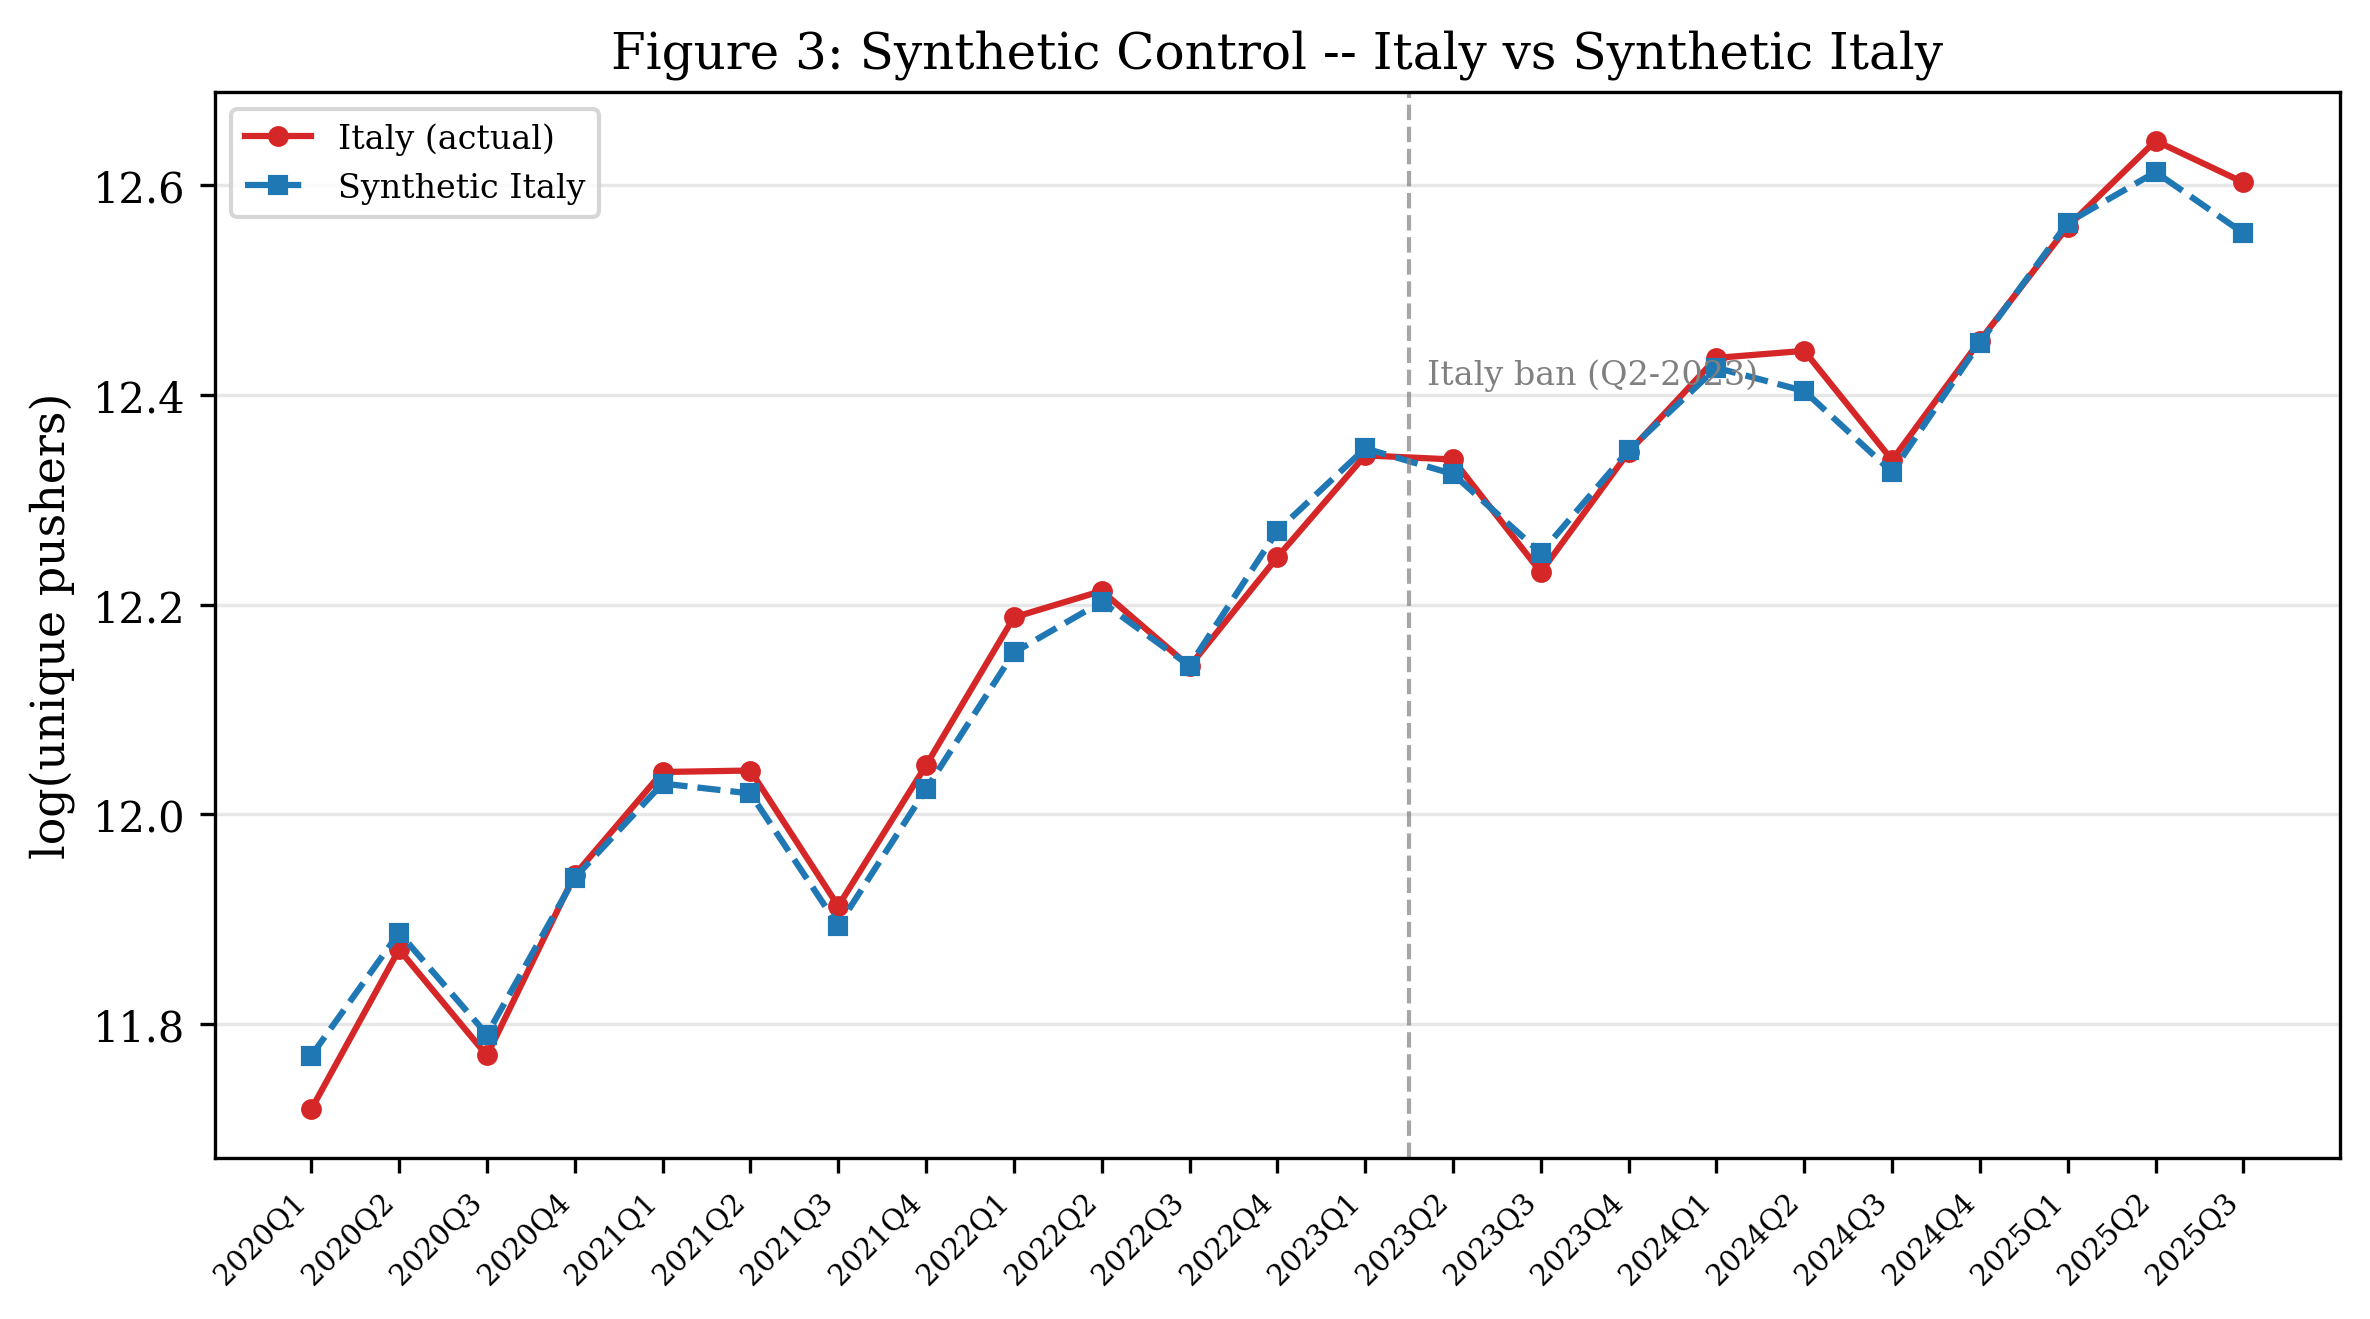
\includegraphics[width=0.8\textwidth]{figures/fig3_synthetic_control_italy.png}
    \caption{Synthetic Control: Italy vs. Synthetic Italy. The dashed vertical line marks Italy's ChatGPT ban (Q2 2023). Pre-treatment RMSPE = 0.023. Post-ban gap = +0.013 (no effect).}
    \label{fig:scm}
\end{figure}

\section{Robustness}

Table \ref{tab:robust} summarizes our robustness battery.

\textbf{Placebo outcome.} Using the number of programming languages (which should not be affected by ChatGPT access) as the outcome, we find a coefficient of $-0.166$ ($p = 0.062$). This borderline result is a concern---it suggests that restricted countries may be diverging on dimensions beyond ChatGPT's influence.

\textbf{Placebo timing.} Assigning a fake treatment date of Q2 2021 and restricting the sample to the pre-ChatGPT period yields a coefficient of $-0.002$ ($p = 0.993$), confirming no divergence before ChatGPT existed.

\textbf{Excluding COVID.} Dropping all 2020 observations and re-running yields $-0.398$ ($p = 0.024$), which is statistically significant. The COVID period may have introduced noise that inflated standard errors in the full sample.

\textbf{OECD-only controls.} Restricting the control group to OECD countries yields $-0.026$ ($p = 0.922$)---effectively zero. This is an important finding: the effect is driven by comparison against developing countries, not against comparable economies. This raises the concern that the result reflects divergent development trajectories rather than ChatGPT-specific effects.

\begin{table}[H]
\centering
\begin{threeparttable}
\caption{Robustness Checks}
\label{tab:robust}
\small
\begin{tabular}{lccc}
\toprule
Specification & Coefficient & SE & $p$-value \\
\midrule
Baseline & $-$0.389 & 0.260 & 0.135 \\
Placebo outcome (N languages) & $-$0.166 & 0.089 & 0.062 \\
Placebo timing (Q2 2021) & $-$0.002 & 0.247 & 0.993 \\
China only & $-$1.386 & 0.036 & $<$0.001 \\
Russia only & $-$0.549 & 0.036 & $<$0.001 \\
Exclude COVID (2020) & $-$0.398 & 0.176 & 0.024 \\
OECD-only controls & $-$0.026 & 0.260 & 0.922 \\
Exclude small countries & $-$0.381 & 0.259 & 0.142 \\
Permutation test & $-$0.389 & 0.207 & 0.006 \\
\bottomrule
\end{tabular}
\begin{tablenotes}
\small
\item \textit{Notes}: All specifications include country and quarter fixed effects with country-clustered SEs. Permutation test based on 500 random assignments of banned status to 5 countries.
\end{tablenotes}
\end{threeparttable}
\end{table}

\section{Discussion}

\subsection{Interpreting the Evidence}

Our findings present a mixed picture. The point estimate is consistently negative across specifications, the permutation test is highly significant, and country-specific estimates for China and Russia are large and precisely estimated. At the same time, pre-trends are formally rejected, the OECD comparison is null, and the placebo outcome is borderline significant.

We interpret the evidence as \textit{suggestive but not definitive} that ChatGPT access restrictions reduce open-source developer activity. The growing gap documented in the event study is consistent with cumulative disadvantage from AI exclusion, but we cannot rule out that other factors---particularly the Russia-Ukraine war and China's tech crackdown---are driving the divergence.

\subsection{Mechanisms}

Several mechanisms could explain why restricted countries show fewer pushers:

\begin{enumerate}
    \item \textbf{Direct productivity loss:} Without ChatGPT, developers are less productive and produce fewer commits, reducing the extensive margin of pushers.
    \item \textbf{Platform migration:} Chinese developers may shift to Gitee (China's domestic GitHub alternative), reducing GitHub-measured activity without reducing actual development.
    \item \textbf{Developer emigration:} Russian developers may emigrate post-sanctions, reducing Russia's GitHub presence regardless of ChatGPT access.
    \item \textbf{Sanctions effects:} International sanctions on Russia reduce economic activity broadly, including software development.
\end{enumerate}

We cannot distinguish between these mechanisms with our data. The Italy null result suggests that mechanism 1 alone is insufficient---if direct productivity loss were the main channel, even a short ban should produce a detectable dip at higher-frequency data.

\subsection{Limitations}

\begin{enumerate}
    \item \textbf{Small number of treated units:} With only 5 persistently blocked countries, our DiD is severely underpowered for country-level inference. The permutation test partially addresses this but does not resolve the fundamental identification concern.
    \item \textbf{Pre-trend violation:} The formal rejection of parallel pre-trends ($p = 0.0003$) is a serious identification threat. While individual pre-period coefficients are small, their joint significance suggests systematic pre-existing divergence.
    \item \textbf{Confounders:} We cannot separate ChatGPT effects from Russia-Ukraine war impacts, China's tech policies, VPN circumvention, or platform migration.
    \item \textbf{OECD null:} The effect disappears when comparing against OECD countries, suggesting the result may reflect broader developing-country divergence rather than AI-specific effects.
    \item \textbf{GitHub selection:} Our data captures only public GitHub activity, not the full developer ecosystem.
    \item \textbf{VPN attenuation:} Developers in restricted countries can access ChatGPT via VPNs, making our estimates conservative lower bounds---but also raising the question of whether the ``treatment'' is truly binding.
\end{enumerate}

\section{Conclusion}

We document a growing gap in open-source developer activity between countries with and without ChatGPT access, using policy-imposed restrictions as a natural experiment. Our DiD estimate of $-0.389$ log points, supported by permutation inference ($p = 0.006$) and strong country-specific effects for China ($-1.386$, $p < 0.001$) and Russia ($-0.549$, $p < 0.001$), provides suggestive evidence that AI access restrictions carry real costs for software development ecosystems.

However, the evidence falls short of a definitive causal claim. Pre-trend violations, the OECD null result, and multiple confounders prevent us from isolating ChatGPT's specific contribution. Our paper's primary contribution is methodological: we demonstrate that AI access restrictions create a viable natural experiment for studying AI's economic impact, and we identify the key threats to validity that future research---with higher-frequency data, VPN usage controls, and platform-level alternatives---must address.

For policymakers, the message is cautionary: even if our estimates are attenuated by confounders, the direction is consistently negative and the magnitude is large. Countries considering AI access restrictions should weigh these potential costs against their regulatory objectives.

\singlespacing
\bibliography{references}

\clearpage
\appendix
\section{Additional Figures}

\begin{figure}[H]
    \centering
    
\includegraphics[width=\textwidth]{figures/fig1_raw_trends.png}
    \caption{Raw Trends: Average Log Pushers for Banned vs. Non-Banned Countries. The vertical dashed line marks ChatGPT launch (Q4 2022).}
    \label{fig:rawtrends}
\end{figure}

\begin{figure}[H]
    \centering
    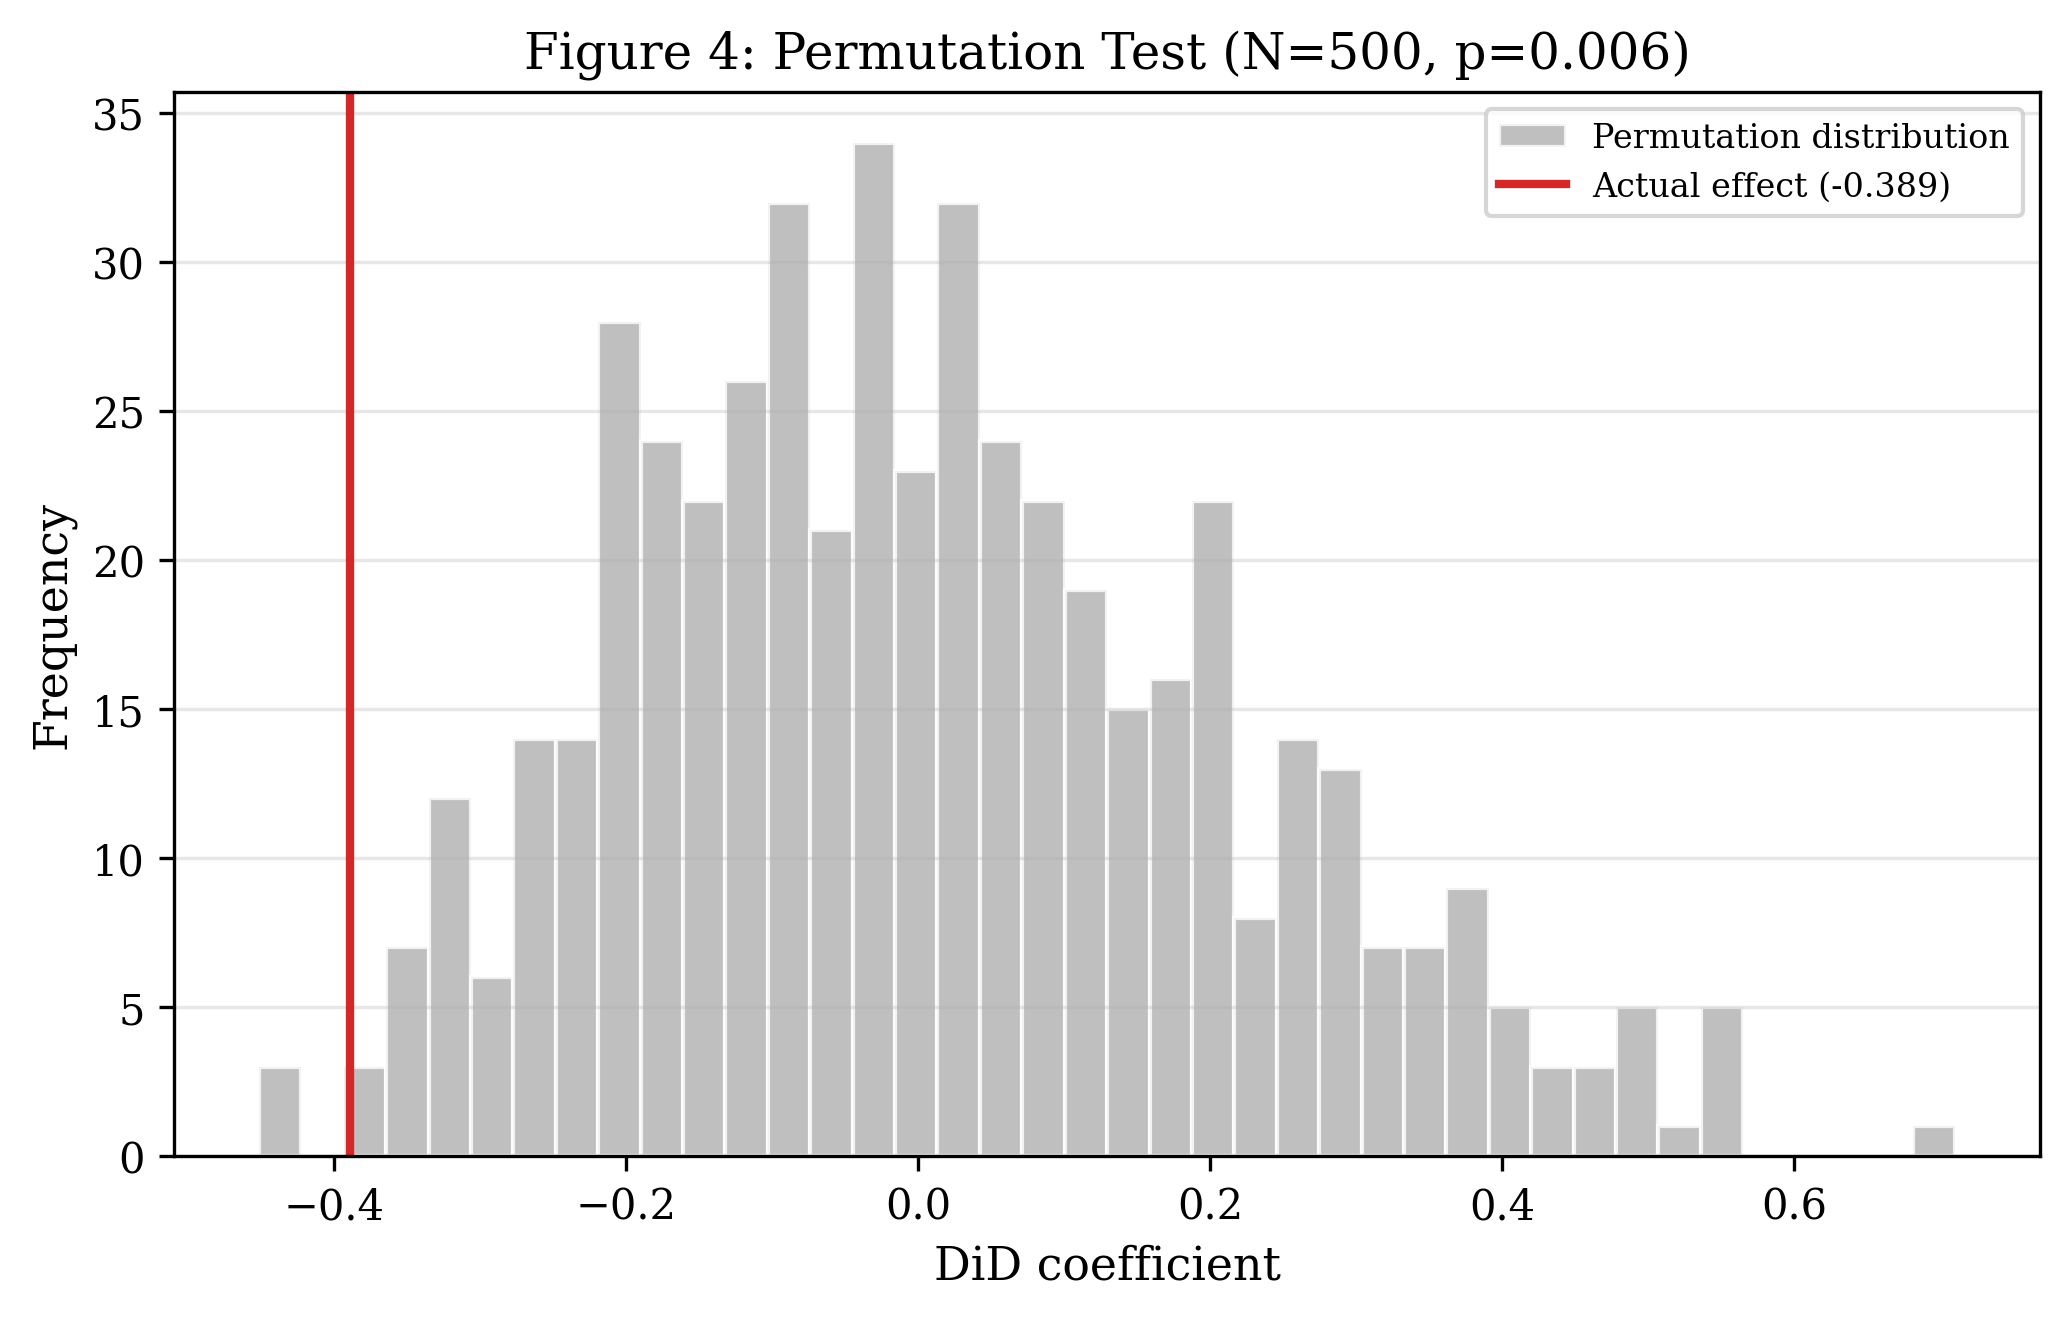
\includegraphics[width=0.8\textwidth]{figures/fig4_permutation_test.png}
    \caption{Permutation Distribution: 500 Random Treatment Assignments. The vertical red line marks the actual DiD estimate ($-0.389$). Permutation $p = 0.006$.}
    \label{fig:permutation}
\end{figure}

\end{document}
